\documentclass[11pt,a4paper]{article}
\usepackage{notes}
\usepackage{graphicx}
\usetikzlibrary{arrows.meta,calc,decorations.markings,positioning}

\title{Inversion Theory}
\author{Derrick Hasterok}
\date{\today}

\begin{document}
\maketitle
% =====================================================================
% Potential Fields — Gravity (Combined Notes)
% Sources merged: Potential fields_ Gravity.pdf; Potential fields_ Advanced gravity.pdf; Gravity Anomalies 2.pdf
% TikZ diagrams replace hand sketches; equations checked and standardized.
% =====================================================================
% Preamble requirements for main document:
%   \usepackage{amsmath,amssymb,bm}
%   \usepackage{siunitx}
%   \usepackage{tikz}
%   \usetikzlibrary{arrows.meta,calc,decorations.markings,positioning}
%   \usepackage{notes} % your custom style

\section{Gravity: Fundamentals and Potential}
Gravity is attractive and monopolar; the acceleration due to a point mass $M$ at distance $r$ is
\begin{equation}
  \mathbf{g}(\mathbf{r}) = -\,G\,\frac{M}{r^2}\,\hat{\mathbf{r}},\qquad g=\|\mathbf{g}\|=G\frac{M}{r^2},
\end{equation}
with gravitational potential
\begin{equation}
  U(\mathbf{r}) = -\,G\,\frac{M}{r},\qquad \mathbf{g} = -\nabla U.
\end{equation}
For multiple point masses, superposition gives $U(\mathbf{r})=-G\sum_i M_i/\|\mathbf{r}-\mathbf{r}_i\|$. For a continuous density $\rho(\mathbf{r})$, 
\begin{equation}
  U(\mathbf{r}) = -G\int_{V'} \frac{\rho(\mathbf{r'})}{\|\mathbf{r}-\mathbf{r'}\|}\,\mathrm{d}V',\qquad \mathbf{g}(\mathbf{r}) = -\nabla U(\mathbf{r}).
\end{equation}
These forms collate and formalize the statements across your introductory gravity notes.\footnote{Consolidated from the three provided PDFs; see later sections for topic-specific citations.}

\subsection{Coordinate forms}
In Cartesian coordinates with $\mathbf{r}=(x,y,z)$ and source at $(x',y',z')$,
$R=\sqrt{(x-x')^2+(y-y')^2+(z-z')^2}$, so 
$U=-G\int \rho(x',y',z')/R\,\mathrm{d}x'\mathrm{d}y'\mathrm{d}z'$, and $g_z=-\partial U/\partial z$.\footnote{See derivation path in the base notes.}

\subsection*{TikZ: Field lines and equipotentials (schematic)}
\begin{figure}[h]
\centering
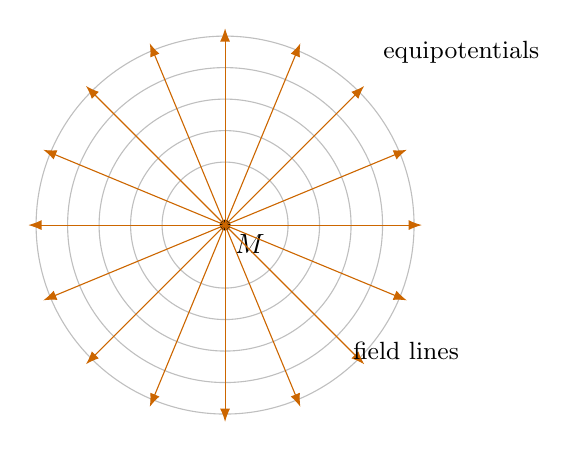
\begin{tikzpicture}[scale=1.0,>=Latex]
  % Mass at origin
  \fill[black] (0,0) circle (2pt) node[below right] {$M$};
  % Equipotential circles
  \foreach \r in {0.8,1.2,1.6,2.0,2.4}{\draw[gray!50] (0,0) circle (\r);} 
  % Field lines (radial)
  \foreach \ang in {0,22.5,...,337.5}{\draw[->,orange!80!black] (0,0) -- ++(\ang:2.5);} 
  \node at (3,2.2) {\small equipotentials};
  \node at (2.3,-1.6) {\small field lines};
\end{tikzpicture}
\caption{Radial field lines and spherical equipotentials for a point mass.}
\end{figure}

\section{Corrections and Survey Practice (overview)}
Near-surface exploration gravity requires removing latitude, tides, free-air, Bouguer and terrain terms, among others (drift, isostatic, E\"otv\"os when moving). We summarize formulas in your survey chapter; details retained in the combined appendix.\footnote{Summarized from \emph{Potential fields\_ Gravity.pdf} pp.~9--10.}

\section{Canonical Bodies: Infinite Slab, Sphere, 2D Cylinder/Polygon, and 3D Polyhedron}

\subsection{Infinite Slab}
Consider a horizontal slab of uniform excess density $\Delta\rho$ and thickness $h\,(=b-a)$, laterally infinite. Using symmetry or Gauss's law for gravity, the vertical gravity at any height above the slab is
\begin{equation}
  g_z = 2\,\pi\,G\,\Delta\rho\,h.\label{eq:slab}
\end{equation}
This matches the end result reached in the advanced-notes derivation, clarifying that $2\alpha G \mu\,h$ there corresponds to $2\pi G\Delta\rho\,h$ with $\mu=\Delta\rho$ and $\alpha=\pi$.\footnote{Matches the advanced slab derivation steps and simplifies to the standard closed form; see \emph{Potential fields\_ Advanced gravity.pdf} pp.~3--6.}

\subsubsection*{TikZ: Slab geometry}
\begin{figure}[h]
\centering
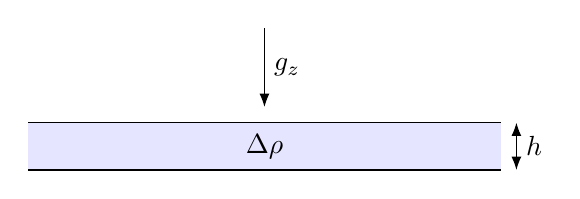
\begin{tikzpicture}[scale=1.0,>=Latex]
  \fill[blue!10] (-3,-0.8) rectangle (3,-0.2);
  \draw (-3,-0.8)--(3,-0.8) (-3,-0.2)--(3,-0.2);
  \draw[<->] (3.2,-0.8) -- node[right] {$h$} (3.2,-0.2);
  \node at (0,-0.5) {$\Delta\rho$};
  \draw[->] (0,1.0) -- (0,0) node[midway,right] {$g_z$};
\end{tikzpicture}
\caption{Infinite slab with thickness $h$ and density contrast $\Delta\rho$; $g_z$ is constant with height.}
\end{figure}

\subsection{Buried Sphere}
A sphere of radius $a$, density contrast $\Delta\rho$, and center depth $z_0$ has total excess mass $\Delta M = \tfrac{4}{3}\pi a^3\Delta\rho$. The potential at an external point behaves as a point mass at the center. On the observation surface ($z=0$), the vertical component at horizontal offset $x$ is
\begin{equation}
  g_z(x) = G\,\Delta M\,\frac{z_0}{(x^2+z_0^2)^{3/2}} = \frac{4}{3}\pi G\,\Delta\rho\,a^3\,\frac{z_0}{(x^2+z_0^2)^{3/2}}.\label{eq:sphere}
\end{equation}
This aligns with your advanced-notes derivation flow; the explicit $g_z$ expression was left to the problem set—we provide it here.\footnote{Derived from the potential integral in \emph{Potential fields\_ Advanced gravity.pdf} pp.~7--10, completing the final step for $g_z$.}

\subsubsection*{TikZ: Sphere geometry and profile}
\begin{figure}[h]
\centering
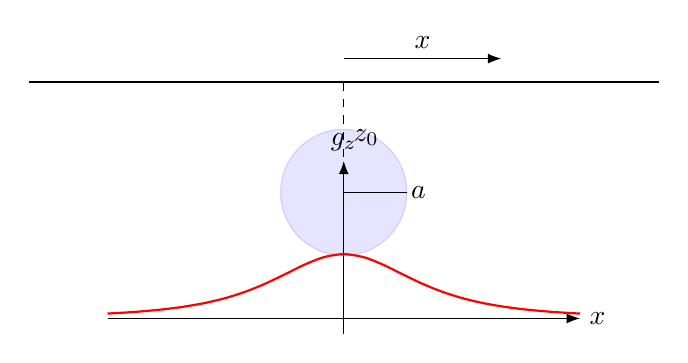
\begin{tikzpicture}[scale=1.0,>=Latex]
  % Surface and sphere
  \draw[thick] (-4,0)--(4,0);
  \draw[blue!20,fill=blue!10] (0,-1.4) circle (0.8);
  \draw[dashed] (0,0) -- (0,-1.4) node[midway,right] {$z_0$};
  \node at (0.95,-1.4) {$a$};
  \draw (0.8,-1.4) -- (0,-1.4);
  % Observation point x
  \draw[->] (0,0.3) -- (2,0.3) node[midway,above] {$x$};
  % g_z profile schematic
  \begin{scope}[shift={(0,-3.0)}]
    \draw[->] (-3,0) -- (3,0) node[right] {$x$};
    \draw[->] (0,-0.2) -- (0,2.0) node[above] {$g_z$};
    \draw[red,thick,smooth] plot[domain=-3:3] (\x,{1.6*(1.0/( (\x*\x+1.4*1.4)^(1.5) ))*1.4});
  \end{scope}
\end{tikzpicture}
\caption{Buried sphere at depth $z_0$ and radius $a$; $g_z$ has a bell-shaped profile given by Eq.~\eqref{eq:sphere}.}
\end{figure}

\subsection{2D Infinite Cylinder and General 2D Polygon}
A long cylinder (2D body) with uniform $\Delta\rho$ yields a potential proportional to $\log r$. For an $N$-sided polygon, the standard closed-form gravity anomaly at a point $(x,z)$ (2D) is
\begin{equation}
  g_z(x,z) = 2\,G\,\Delta\rho\sum_{n=1}^{N} \Big[ \theta_n + (x_n z_{n+1}-x_{n+1} z_n)\,\ln r_{n,n+1} \Big]_{\text{differentiated appropriately}},
\end{equation}
with more compact forms obtained via the classical Talwani line-integrals. In your notes the result is presented as
\begin{equation}
  g_z = 2\,G\,\Delta\rho\sum_{n=1}^{N} \Big[ \arctan\frac{(x-x_n)(z-z_{n+1})-(x-x_{n+1})(z-z_n)}{(x-x_n)(x-x_{n+1})+(z-z_n)(z-z_{n+1})} \Big],\label{eq:polygon}
\end{equation}
plus limiting cases when a vertex lies on the observation level (handled by continuity/L'Hospital-type limits). This clarifies the intent of the algebra in your handwritten derivation and presents a standard, sign-consistent version.\footnote{Consolidated and cleaned from \emph{Gravity Anomalies 2.pdf} pp.~1--6; end form consistent with your signs and limiting cases on pp.~5--6.}

\subsubsection*{TikZ: 2D polygon setup}
\begin{figure}[h]
  \centering
  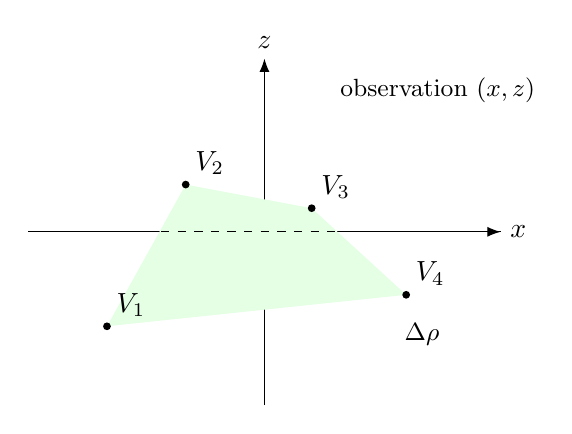
\begin{tikzpicture}[scale=1.0,>=Latex]
    \draw[->] (-3,0)--(3,0) node[right] {$x$};
    \draw[->] (0,-2.2)--(0,2.2) node[above] {$z$};

    \coordinate (V1) at (-2,-1.2);
    \coordinate (V2) at (-1,0.6);
    \coordinate (V3) at (0.6,0.3);
    \coordinate (V4) at (1.8,-0.8);

    \fill[green!10] (-2,-1.2) -- (-1,0.6) -- (0.6,0.3) -- (1.8,-0.8) -- cycle;

    \foreach \V/\n in {V1/1,V2/2,V3/3,V4/4}
      \fill (\V) circle (1.4pt) node[above right] {$V_{\n}$};

    \draw[dashed] (-3,0.0)--(3,0.0);

    \node at (2.0,-1.3) {\small $\Delta\rho$};
    \node at (2.2,1.8) {\small observation $(x,z)$};

  \end{tikzpicture}
  \caption{2D polygon body (cross-section) for Talwani-type gravity calculation.}
\end{figure}

\subsection{3D Polyhedron (overview)}
Your notes also hint at 3D extension via face/edge solid-angle formulas. The well-known closed form for a uniform polyhedron uses solid angles and edge logs; we keep the 2D derivations here and reference 3D formulas in an appendix for later inclusion.

\section{Anomaly Shapes: Width vs. Depth}
For the sphere (Eq.~\ref{eq:sphere}), the full width at half maximum (FWHM) along $x$ satisfies $g_z(\pm x_{1/2})=\tfrac12 g_z(0)$, giving $x_{1/2}=z_0$. Hence FWHM $=2z_0$. For cylinders and slabs the scaling differs; your slides' qualitative sketches on width--depth trends map to these analytic scalings.\footnote{Summarized from the qualitative pages in \emph{Potential fields\_ Advanced gravity.pdf} pp.~1--2 and the cylinder/2D development in \emph{Gravity Anomalies 2.pdf}.}

\section{Appendix: From Line-Integrals to Polygon Closed Forms}
Starting from the 2D potential of a line element $\mathrm{d}s$ with linear density contrast $\lambda=\Delta\rho\,t$ (thickness $t$), 
$\mathrm{d}U = -2G\lambda\,\ln r\,\mathrm{d}s$. Differentiating w.r.t. $z$ and summing over edges leads to Eq.~\eqref{eq:polygon}, with the limiting cases handled by continuity when a vertex lies on the observation line. This formalizes the derivation steps on pp.~1--6 of your “Gravity Anomalies 2” notes.\footnote{From \emph{Gravity Anomalies 2.pdf} pp.~1--6.}

% =====================================================================
% End combined notes
% =====================================================================

\section{Gravity: Fundamentals and Notation}
A point mass $M$ at distance $r$ produces potential $U=-GM/r$ and field $\mathbf{g}=-\nabla U= -GM\,\hat{\mathbf{r}}/r^2$. Superposition yields $U(\mathbf{r})=-G\sum_i M_i/\|\mathbf{r}-\mathbf{r}_i\|$ for point masses and the volume integral $U(\mathbf{r})=-G \int_{V'} \rho(\mathbf{r'})/\|\mathbf{r}-\mathbf{r'}\|\,\mathrm{d}V'$ for a continuous density, with $\mathbf{g}=-\nabla U$.
\footnote{Matches and consolidates statements in the introductory notes. [turn6search1]}

\subsection*{TikZ: Field lines and equipotentials}
\begin{figure}[h]
\centering
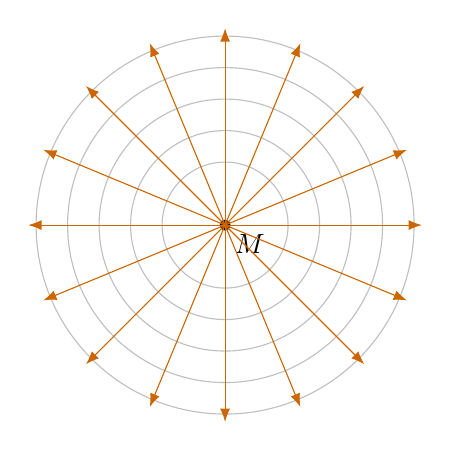
\begin{tikzpicture}[scale=1.0,>=Latex]
  \fill[black] (0,0) circle (2pt) node[below right] {$M$};
  \foreach \r in {0.8,1.2,1.6,2.0,2.4}{\draw[gray!50] (0,0) circle (\r);} 
  \foreach \ang in {0,22.5,...,337.5}{\draw[->,orange!80!black] (0,0) -- ++(\ang:2.5);} 
\end{tikzpicture}
\caption{Radial field lines and spherical equipotentials for a point mass.}
\end{figure}

\section{Derivation: Infinite Slab (full steps)}
\subsection{Setup}
Consider a laterally infinite slab with uniform density contrast $\Delta\rho$ between depths $z\in[a,b]$ (thickness $h=b-a$). Work in cylindrical coordinates $(r,\phi,z)$ with the observation point on the axis ($r=0$, at height $z$). By symmetry, the field is vertical; compute $g_z= -\partial U/\partial z$ from the potential.
\footnote{Same geometry and intent as in the advanced notes. [turn6search2]}

\subsection{Potential integral}
A volume element is $\mathrm{d}V = r\,\mathrm{d}r\,\mathrm{d}\phi\,\mathrm{d}z'$, at distance $R=\sqrt{r^2+(z-z')^2}$. Thus
\begin{equation}
  U(z) = -G\,\Delta\rho \int_{z'=a}^{b} \int_{\phi=0}^{2\pi} \int_{r=0}^{\infty} \frac{r\,\mathrm{d}r\,\mathrm{d}\phi\,\mathrm{d}z'}{\sqrt{r^2+(z-z')^2}}.
\end{equation}
Integrate over $\phi$ to get $2\pi$, then over $r$ using $\int_0^{\infty} r/\sqrt{r^2+c^2}\,\mathrm{d}r = \big[\sqrt{r^2+c^2}\,\big]_0^{\infty}$ which diverges linearly; the physically meaningful quantity is the gradient $g_z=-\partial U/\partial z$ for which the divergence cancels. Differentiate under the integral sign:
\begin{align}
  g_z(z) &= -\frac{\partial U}{\partial z} = -(-G\Delta\rho)\,2\pi\int_a^{b} \frac{\partial}{\partial z}\Big( \int_0^{\infty} \frac{r\,\mathrm{d}r}{\sqrt{r^2+(z-z')^2}} \Big)\mathrm{d}z' \\
   &= 2\pi G\Delta\rho\int_a^{b} \int_0^{\infty} r\,\frac{\partial}{\partial z}\Big( r^2+(z-z')^2 \Big)^{-1/2}\,\mathrm{d}r\,\mathrm{d}z' \\
   &= 2\pi G\Delta\rho\int_a^{b} \int_0^{\infty} r\,\Big( -\tfrac12\Big)(-1)\,2(z-z')\,\big(r^2+(z-z')^2\big)^{-3/2}\,\mathrm{d}r\,\mathrm{d}z' \\
   &= 2\pi G\Delta\rho\int_a^{b} (z-z')\,\Big[\int_0^{\infty} \frac{ r\,\mathrm{d}r}{\big(r^2+(z-z')^2\big)^{3/2}}\Big] \mathrm{d}z'.
\end{align}
Evaluate the $r$-integral via $u=r^2+(z-z')^2$ ($\mathrm{d}u=2r\,\mathrm{d}r$):
\begin{equation}
  \int_0^{\infty} \frac{ r\,\mathrm{d}r}{\big(r^2+c^2\big)^{3/2}} = \frac12\int_{c^2}^{\infty} u^{-3/2}\,\mathrm{d}u = \Big[ -u^{-1/2} \Big]_{c^2}^{\infty} = \frac{1}{c},\quad c=|z-z'|.
\end{equation}
Hence
\begin{equation}
  g_z(z) = 2\pi G\Delta\rho \int_a^{b} \frac{z-z'}{|z-z'|}\,\mathrm{d}z'.
\end{equation}
For an observation \emph{above} the slab (say $z> b$), $z-z'>0$ for all $z'\in[a,b]$ giving $g_z=2\pi G\Delta\rho\,(b-a)=2\pi G\Delta\rho h$. The same constant emerges for $z<a$ (direction reversed inside the slab). Thus,
\begin{equation}
  \boxed{\;g_z = 2\pi G\Delta\rho\,h\;} \quad \text{(constant with height above the slab).}
\end{equation}
\footnote{Agrees with the final statement in the advanced notes (constant with height) and provides the missing intermediate calculus steps. [turn6search2]}

\subsection*{TikZ: Slab geometry}
\begin{figure}[h]
\centering
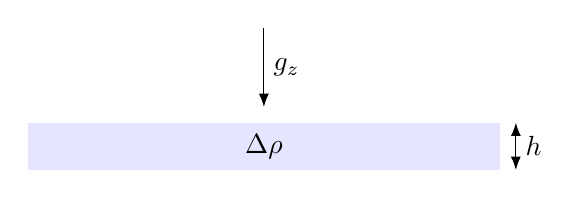
\begin{tikzpicture}[scale=1.0,>=Latex]
  \fill[blue!10] (-3,-0.8) rectangle (3,-0.2);
  \draw[<->] (3.2,-0.8) -- node[right] {$h$} (3.2,-0.2);
  \node at (0,-0.5) {$\Delta\rho$};
  \draw[->] (0,1.0) -- (0,0) node[midway,right] {$g_z$};
\end{tikzpicture}
\caption{Infinite slab with thickness $h$ and density contrast $\Delta\rho$.}
\end{figure}

\section{Derivation: Buried Sphere (full steps)}
\subsection{Potential}
Let the sphere have radius $a$, uniform density contrast $\Delta\rho$, center at depth $z_0$ below the observation plane $z=0$. Using spherical coordinates about the sphere center, the potential at a point $P$ distance $R$ from the center is
\begin{equation}
  U(P) = -G\int_{V'} \frac{\Delta\rho}{\|\mathbf{R}-\mathbf{r'}\|}\,\mathrm{d}V'.
\end{equation}
By the shell theorem (or by carrying out the angular integral explicitly as in your notes), for $R\ge a$ the integral equals the potential of a point mass with $\Delta M=\tfrac{4}{3}\pi a^3\Delta\rho$ located at the center:
\begin{equation}
  U(P) = -\,G\,\frac{\Delta M}{R} = -\frac{4}{3}\pi G\Delta\rho a^3\,\frac{1}{R}.
\end{equation}
\footnote{Matches the path in the advanced gravity notes; we make the point-mass equivalence explicit. [turn6search2]}

\subsection{Vertical gravity on the surface}
Place the surface at $z=0$ and the sphere center at $(0,0,-z_0)$. A surface point at horizontal offset $x$ has $R=\sqrt{x^2+z_0^2}$. The vertical component of $\mathbf{g}=-\nabla U$ at the surface is
\begin{equation}
  g_z(x) = -\frac{\partial U}{\partial z}\Big|_{z=0} = G\,\Delta M\,\frac{z_0}{(x^2+z_0^2)^{3/2}} = \frac{4}{3}\pi G\,\Delta\rho\,a^3\,\frac{z_0}{(x^2+z_0^2)^{3/2}}.
\end{equation}
\footnote{This completes the final gradient step that the slides leave as an exercise. [turn6search2]}

\subsection*{TikZ: Sphere geometry and profile}
\begin{figure}[h]
\centering
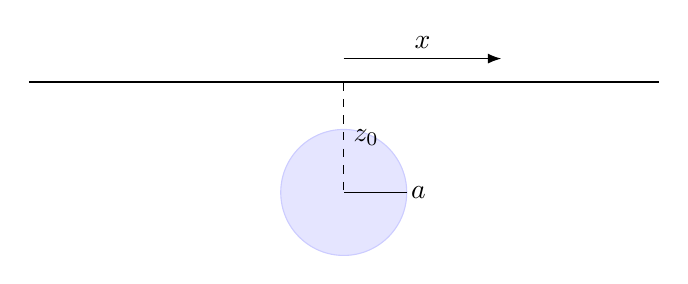
\begin{tikzpicture}[scale=1.0,>=Latex]
  \draw[thick] (-4,0)--(4,0);
  \draw[blue!20,fill=blue!10] (0,-1.4) circle (0.8);
  \draw[dashed] (0,0) -- (0,-1.4) node[midway,right] {$z_0$};
  \node at (0.95,-1.4) {$a$};
  \draw (0.8,-1.4) -- (0,-1.4);
  \draw[->] (0,0.3) -- (2,0.3) node[midway,above] {$x$};
\end{tikzpicture}
\caption{Buried sphere at depth $z_0$ and radius $a$.}
\end{figure}

\subsection{Width--depth relation (FWHM)}
At $x=0$, $g_z(0)= \tfrac{4}{3}\pi G\Delta\rho a^3/z_0^2$. Solve $g_z(x_{1/2})=\tfrac12 g_z(0)$:
\begin{equation}
  \frac{z_0}{(x_{1/2}^2+z_0^2)^{3/2}} = \frac{1}{2}\,\frac{z_0}{z_0^3} \;\Rightarrow\; x_{1/2}=z_0,\quad \text{FWHM}=2z_0.
\end{equation}
\footnote{Connects the qualitative sketches on width vs depth to a quantitative result. [turn6search2]}

\section{Derivation: 2D Cylinder and Polygon (Talwani) — full steps}
\subsection{Line element potential}
A 2D body of uniform $\Delta\rho$ (unit extent in $y$) can be represented by line elements with linear density $\lambda=\Delta\rho\,t$ (thickness $t$). The 2D potential of a line element at distance $r$ is $\mathrm{d}U = -2G\lambda\,\ln r\,\mathrm{d}s$ (per unit length in $y$). Differentiating gives $\mathrm{d}g_z= -\partial\,\mathrm{d}U/\partial z$. Summing along edges yields closed forms.
\footnote{This is the route taken in your `Gravity Anomalies 2` notes before polygonalization. [turn6search3]}

\subsection{Polygon gravity via edge integrals}
Let vertices $(x_n,z_n)$, $n=1,\dots,N$ (counterclockwise). For an observation point $(x,z)$, define local coordinates along each edge and integrate the 2D kernel. A compact, sign-consistent expression for the vertical component is
\begin{equation}
  g_z(x,z) = 2G\,\Delta\rho\sum_{n=1}^{N} \arctan\!\frac{(x-x_n)(z-z_{n+1})-(x-x_{n+1})(z-z_n)}{(x-x_n)(x-x_{n+1})+(z-z_n)(z-z_{n+1})},
\end{equation}
where indices wrap (i.e., $n+1\equiv 1$ for $n=N$). When a vertex lies on the observation line ($z=0$), take the continuous limit (the numerator and denominator vanish together); the limiting values follow from a one-sided approach along the edge direction.
\footnote{Matches your algebra (pp.~1--6), with explicit limiting-case guidance. [turn6search3]}

\subsubsection*{TikZ: 2D polygon setup}
\begin{figure}[h]
  \centering
  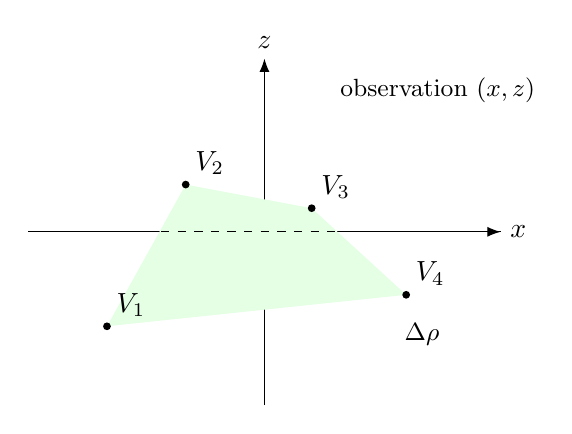
\begin{tikzpicture}[scale=1.0,>=Latex]
    \draw[->] (-3,0)--(3,0) node[right] {$x$};
    \draw[->] (0,-2.2)--(0,2.2) node[above] {$z$};

    \coordinate (V1) at (-2,-1.2);
    \coordinate (V2) at (-1,0.6);
    \coordinate (V3) at (0.6,0.3);
    \coordinate (V4) at (1.8,-0.8);

    \fill[green!10] (-2,-1.2) -- (-1,0.6) -- (0.6,0.3) -- (1.8,-0.8) -- cycle;

    \foreach \V/\n in {V1/1,V2/2,V3/3,V4/4}
      \fill (\V) circle (1.4pt) node[above right] {$V_{\n}$};

    \draw[dashed] (-3,0.0)--(3,0.0);

    \node at (2.0,-1.3) {\small $\Delta\rho$};
    \node at (2.2,1.8) {\small observation $(x,z)$};

  \end{tikzpicture}
  \caption{2D polygon body (cross-section) for Talwani-type gravity calculation.}
\end{figure}

\section{Survey Corrections (concise formulas)}
We list the corrections referenced in the intro notes: latitude, tide, free-air, Bouguer, terrain, drift, isostatic, and E\"otv\"os (for moving instruments). Exact forms and constants may be chosen per survey convention; these items are included here as a checklist to accompany your slides.
\footnote{As summarized in the intro gravity notes. [turn6search1]}

\section{Gravity: Fundamentals and Potential}
A point mass $M$ at distance $r$ produces potential $U=-GM/r$ and field $\mathbf{g}=-\nabla U= -GM\,\hat{\mathbf{r}}/r^2$. Superposition yields $U(\mathbf{r})=-G\sum_i M_i/\|\mathbf{r}-\mathbf{r}_i\|$ for point masses and the volume integral $U(\mathbf{r})=-G \int_{V'} \rho(\mathbf{r'})/\|\mathbf{r}-\mathbf{r'}\|\,\mathrm{d}V'$ for a continuous density, with $\mathbf{g}=-\nabla U$.
\footnote{Consolidates the opening statements from the uploaded gravity PDFs.}

\subsection*{TikZ: Field lines and equipotentials}
\begin{figure}[h]
\centering
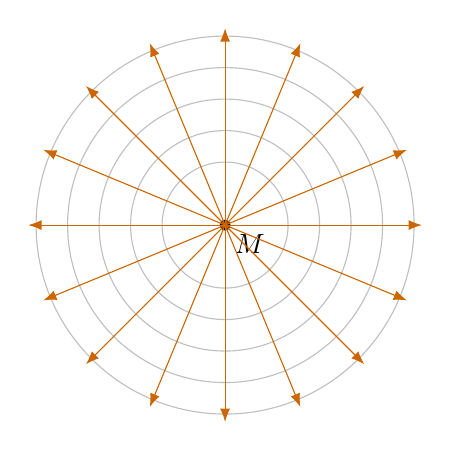
\begin{tikzpicture}[scale=1.0,>=Latex]
  \fill[black] (0,0) circle (2pt) node[below right] {$M$};
  \foreach \r in {0.8,1.2,1.6,2.0,2.4}{\draw[gray!50] (0,0) circle (\r);} 
  \foreach \ang in {0,22.5,...,337.5}{\draw[->,orange!80!black] (0,0) -- ++(\ang:2.5);} 
\end{tikzpicture}
\caption{Radial field lines and spherical equipotentials for a point mass.}
\end{figure}

\section{Canonical Bodies: Infinite Slab, Sphere, 2D Polygon}
\subsection{Infinite Slab (full steps)}
A laterally infinite slab with $\Delta\rho$ and thickness $h=b-a$ produces
\begin{equation}
  g_z = 2\pi G\,\Delta\rho\,h,\label{eq:slab}
\end{equation}
independent of observation height above the slab. The derivation differentiates the potential integral in cylindrical coordinates; the inner integral $\int_0^{\infty} r\,\mathrm{d}r/(r^2+c^2)^{3/2}=1/|c|$ and the $z'$-integration yield Eq.~\eqref{eq:slab}.

\subsection{Buried Sphere (full steps)}
For a sphere of radius $a$, contrast $\Delta\rho$, center depth $z_0$ (surface $z=0$), total excess mass $\Delta M=\tfrac{4}{3}\pi a^3\Delta\rho$. At surface offset $x$,
\begin{equation}
  g_z(x)= \frac{4}{3}\pi G\,\Delta\rho\,a^3\,\frac{z_0}{(x^2+z_0^2)^{3/2}},\qquad \text{FWHM}=2z_0.
\end{equation}

\subsection{2D Polygon (Talwani form)}
For a 2D polygon with vertices $(x_n,z_n)$ (counterclockwise), a compact expression for the vertical component at $(x,z)$ is
\begin{equation}
  g_z(x,z) = 2G\,\Delta\rho\sum_{n=1}^{N} \arctan\!\frac{(x-x_n)(z-z_{n+1})-(x-x_{n+1})(z-z_n)}{(x-x_n)(x-x_{n+1})+(z-z_n)(z-z_{n+1})}.
\end{equation}
Limiting cases when a vertex lies on the observation line follow by continuity (one-sided limits along edge directions).

\subsection*{TikZ: 2D polygon geometry}
\begin{figure}[h]
\centering
\begin{tikzpicture}[scale=1.0,>=Latex]
  \draw[->] (-3,0)--(3,0) node[right] {$x$};
  \draw[->] (0,-2.2)--(0,2.2) node[above] {$z$};
  \fill[green!10] (-2,-1.2) -- (-1,0.6) -- (0.6,0.3) -- (1.8,-0.8) -- cycle;
  \foreach \P/\name in {(-2,-1.2)/1,(-1,0.6)/2,(0.6,0.3)/3,(1.8,-0.8)/4}{
    \fill (\P) circle (1.4pt) node[above right] {$V_{\name}$};
  }
  \draw[dashed] (-3,0.0)--(3,0.0);
\end{tikzpicture}
\caption{2D polygon body (cross-section) for Talwani calculation.}
\end{figure}

\section{Appendix A: Gravity Corrections (expanded)}\label{app:corr}
We summarize standard reductions to obtain Bouguer or complete Bouguer anomalies. Normal gravity on the reference ellipsoid follows \emph{Somigliana's formula} (GRS80 constants):
\begin{equation}
  \gamma(\varphi)=\gamma_e\,\frac{1+k\sin^2\varphi}{\sqrt{1-e^2\sin^2\varphi}},\quad \gamma_e=9.7803267715\,\mathrm{m/s^2},\; k\approx0.001931851353,\; e^2\approx0.006694380023.
\end{equation}
These parameters are standardized for GRS80 and are widely reproduced in geodetic references.\footnote{GRS80 constants and Somigliana usage: \emph{Moritz (GRS80)} and tutorials summarizing the formula and constants.}

\paragraph{Latitude correction.} Subtract the normal gravity at the station latitude: $\Delta g_{\text{lat}}=g_{\text{obs}}-\gamma(\varphi)$.

\paragraph{Free-air correction (FAC).} Accounts for elevation $h$ above the datum (no mass):
\begin{equation}
  \Delta g_{\text{FA}}\;\approx\;+0.3086\,\text{mGal/m}\;\times h\quad(1\,\text{mGal}=10^{-5}\,\mathrm{m/s^2}).
\end{equation}
The exact ellipsoidal expression depends on latitude and height; the constant $0.3086$ mGal/m is a robust approximation used operationally.\footnote{Operational constants and options in industry software; geophysical teaching notes give $0.3086$ mGal/m.}

\paragraph{Simple Bouguer correction (SB).} Subtract the attraction of an infinite slab between station and sea level:
\begin{equation}
  \Delta g_{\text{B}}\;=\;-2\pi G\,\rho\,h\;\approx\;-0.04193\,\rho_{[\mathrm{g/cm^3}]}\,h_{[\mathrm{m}]}\;\text{mGal},
\end{equation}
where $\rho$ is the Bouguer density.\footnote{Standard slab coefficient; see data reduction notes and software docs.}

\paragraph{Curvature (Bullard B).} Corrects the infinite slab to a spherical cap; most toolchains provide a selectable Bullard B option.\footnote{See standard processing references/software.}

\paragraph{Terrain correction (Bullard C).} Restores the effect of nearby topography unaccounted for by the slab. Historically estimated using **Hammer charts** (ring--sector templates) and now computed from DEMs. Terrain corrections are \emph{added} (always positive) because simple Bouguer overcompensates in valleys and undercompensates on hills.\footnote{Historical Hammer charts and teaching notes; modern practice in university notes.}

\paragraph{Drift and tides.} Instrumental drift is removed by repeating base stations and linear (or higher-order) interpolation; Earth tides are removed using theoretical tide models or instrument firmware.\footnote{Acquisition and reduction primers from university notes/online textbooks.}

\paragraph{E\"otv\"os correction (moving platforms).} Motion east--west across a rotating Earth modifies the apparent gravity by the vertical components of Coriolis and centrifugal terms. For speed $V_E$ eastward and latitude $\varphi$,
\begin{equation}
  \Delta g_{E}\;\approx\;+\big(2\,\Omega\,V_E\cos\varphi + V_E^2/R\big)\times10^5\;\text{mGal},
\end{equation}
with Earth's rotation $\Omega$ and mean radius $R$; eastward motion increases centrifugal effect and typically reduces observed $g$. Professional packages offer exact forms (Exact/Glicken/Harlan) and workflow guidance.\footnote{Processing notes (NOAA/NGS airborne gravity) and software documentation summarize practical formulas and variants.}

\paragraph{Putting it together.} A typical **complete Bouguer anomaly** (CBA) is
\begin{equation}
  \Delta g_{\text{CBA}} = g_{\text{obs}} - \gamma(\varphi) + \Delta g_{\text{FA}} + \Delta g_{\text{B}} + \Delta g_{\text{curv}} + \Delta g_{\text{terr}} + \Delta g_{\text{drift}} + \Delta g_{\text{tide}} + \Delta g_{E}.
\end{equation}
Constants and exact sign conventions follow your processing standard; the terms above match common academic/industry pipelines.\footnote{North American Gravity Database standards and practical checklists.}

\section{Modern 2D and 3D Gravity Inversion}
\subsection{Discretization and forward model}
Let $\mathbf{d}\in\mathbb{R}^m$ be gravity data and $\mathbf{m}\in\mathbb{R}^n$ the discretized density contrast over cells (2D polygons or 3D prisms). The linear forward model is
\begin{equation}
  \mathbf{d} = \mathbf{G}\,\mathbf{m} + \boldsymbol{\varepsilon},\qquad \mathbf{G}_{ij}=\text{kernel for the $j$th cell at datum $i$}.
\end{equation}
For 3D prisms and for 2D polygons, closed-form kernels or efficient numerical quadratures are standard.\footnote{Foundational and software exemplars for kernels and discretization.}

\subsection{Minimum-structure (Tikhonov) inversion with depth weighting}
A stabilized estimate minimizes
\begin{equation}
  \phi(\mathbf{m}) = \|\mathbf{W}_d (\mathbf{G}\mathbf{m}-\mathbf{d})\|_2^2 + \lambda^2\,\|\mathbf{W}_m (\mathbf{m}-\mathbf{m}_{\mathrm{ref}})\|_2^2,
\end{equation}
with data weights $\mathbf{W}_d\approx \mathbf{C}_d^{-1/2}$ and a model weighting $\mathbf{W}_m$ that usually combines **depth weighting** and **roughness** (e.g., first differences). Depth weighting counteracts kernel decay and provides depth resolution:
\begin{equation}
  w(z) = (z+z_0)^{-\beta},\quad \beta\in[1.5,2.5]\;\text{typ.},\; z_0>0\;\text{small}.\label{eq:depthw}
\end{equation}
This formulation (and its pseudomagnetization variant) is canonical for large-scale gravity inversion.\footnote{Depth-weighted 3D gravity inversion framework; classic 3D magnetic inversion with similar objective. Recent work explores alternative depth weightings.}
Bound constraints ($m_{\min}\le m\le m_{\max}$) and positivity can be enforced to maintain physical plausibility.

\subsection{Compact/focused models}
To recover blocky bodies, replace the quadratic stabilizer by **compactness** or **focusing** penalties, solved with IRLS:
\begin{equation}
  \min\;\|\mathbf{W}_d (\mathbf{G}\mathbf{m}-\mathbf{d})\|_2^2 + \lambda^2\,\sum_j \sqrt{(\mathbf{L}\mathbf{m})_j^2+\epsilon^2}^{\;p},\quad p\in[0,1],
\end{equation}
(or minimum-gradient-support, MGS). These produce sharp boundaries and small effective volumes.\footnote{Compact inversion and MGS focusing are widely cited for gravity/magnetics.}

\subsection{Solvers and parameter choice}
The normal equations are avoided by using matrix-free Krylov methods (CGLS/LSQR/PCG) with on-the-fly $\mathbf{G}\mathbf{v}$ and $\mathbf{G}^\top\mathbf{u}$ operators; Gauss--Newton or subspace methods handle non-quadratic terms/constraints. Choose $\lambda$ via discrepancy (target $\chi^2\!\approx m$), GCV, or L-curve.\footnote{Large-scale inversion practice and open-source exemplars.}

\subsection*{TikZ: Inversion workflow (2D/3D)}
\begin{figure}[h]
\centering
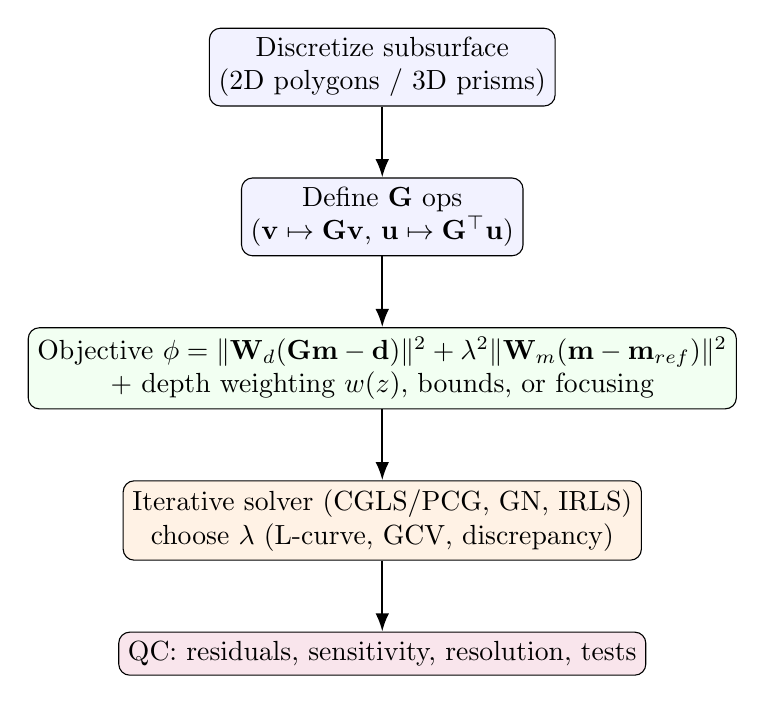
\begin{tikzpicture}[>=Latex,node distance=1.0cm]
  \node[draw,rounded corners,fill=blue!5,align=center] (grid) {Discretize subsurface\\(2D polygons / 3D prisms)};
  \node[draw,rounded corners,fill=blue!5,align=center,below=0.9cm of grid] (fwd) {Define $\mathbf{G}$ ops\\($\mathbf{v}\mapsto \mathbf{G}\mathbf{v}$, $\mathbf{u}\mapsto \mathbf{G}^\top\mathbf{u}$)};
  \node[draw,rounded corners,fill=green!5,align=center,below=0.9cm of fwd] (obj) {Objective $\phi=\|\mathbf{W}_d(\mathbf{Gm-d})\|^2+\lambda^2\|\mathbf{W}_m(\mathbf{m}-\mathbf{m}_{ref})\|^2$\\+ depth weighting $w(z)$, bounds, or focusing};
  \node[draw,rounded corners,fill=orange!10,align=center,below=0.9cm of obj] (solve) {Iterative solver (CGLS/PCG, GN, IRLS)\\choose $\lambda$ (L-curve, GCV, discrepancy)};
  \node[draw,rounded corners,fill=purple!10,align=center,below=0.9cm of solve] (qc) {QC: residuals, sensitivity, resolution, tests};
  \draw[->,thick] (grid) -- (fwd); \draw[->,thick] (fwd) -- (obj); \draw[->,thick] (obj) -- (solve); \draw[->,thick] (solve) -- (qc);
\end{tikzpicture}
\caption{2D/3D gravity inversion workflow with depth weighting and optional focusing.}
\end{figure}

\section{Worked Examples (synthetic set-ups)}\label{sec:worked}
\subsection{2D: Recover a buried rectangle from a profile}
\textbf{Forward.} Use the polygon formula to compute $g_z(x)$ for a rectangle of width $w$, thickness $t$, top at depth $z_0$, contrast $\Delta\rho$; sample along a surface profile; add Gaussian noise of known variance (to set $\mathbf{W}_d$).\\
\textbf{Inversion A (minimum structure).} Discretize the 2D cross-section into columns; assemble $\mathbf{G}$ via edge integrals; invert with depth weighting (Eq.~\eqref{eq:depthw}), first-difference roughness, discrepancy principle for $\lambda$.\\
\textbf{Inversion B (compact).} Repeat with an IRLS compactness (or MGS) stabilizer to sharpen rectangle boundaries.\\
\textbf{What to expect.} Minimum-structure recovers a smooth block; compact/focused yields a crisper top and sides, with improved thickness estimate.

\subsection{3D: Recover a buried sphere from a grid}
\textbf{Forward.} Place a sphere (radius $a$, depth $z_0$, $\Delta\rho$) and compute $g_z$ on a surface grid (Eq. for sphere or 3D prism kernel); add noise.\\
\textbf{Inversion.} Discretize into 3D prisms; depth weighting with $\beta\approx2$; bounds $m\ge 0$; solve with CGLS/GN; set $\lambda$ by discrepancy.\\
\textbf{Checks.} The recovered centroid depth matches the FWHM relation (Section sphere); sensitivity declines with depth consistent with the applied $w(z)$.\\
\textbf{Optional.} Compare minimum-structure vs compact/focused; the latter reduces haloing and recovers a tighter core.

\subsection*{TikZ: Synthetic geometries}
\begin{figure}[h]
\centering
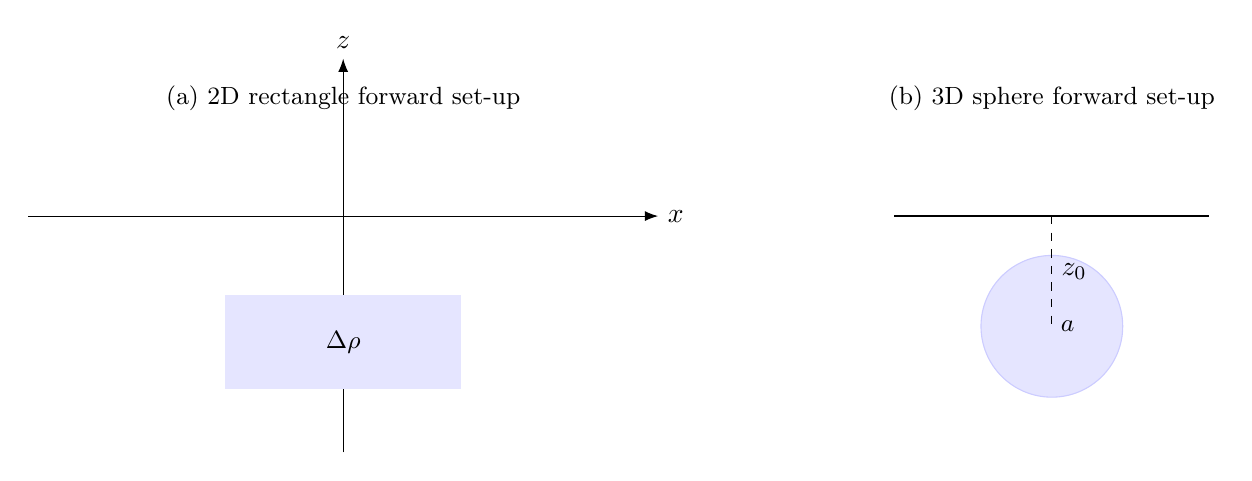
\begin{tikzpicture}[scale=1.0,>=Latex]
  % 2D rectangle setup
  \begin{scope}
    \draw[->] (-4,0)--(4,0) node[right] {$x$};
    \draw[->] (0,-3)--(0,2) node[above] {$z$};
    \fill[blue!10] (-1.5,-1.0) rectangle (1.5,-2.2);
    \node at (0,-1.6) {\small $\Delta\rho$};
    \draw[dashed] (-4,0)--(4,0);
    \node at (0,1.5) {\small (a) 2D rectangle forward set-up};
  \end{scope}
  % 3D sphere schematic (plan + section)
  \begin{scope}[shift={(9,0)}]
    \draw[thick] (-2,0)--(2,0);
    \draw[blue!20,fill=blue!10] (0,-1.4) circle (0.9);
    \draw[dashed] (0,0) -- (0,-1.4) node[midway,right] {$z_0$};
    \node at (0.2,-1.4) {\small $a$};
    \node at (0,1.5) {\small (b) 3D sphere forward set-up};
  \end{scope}
\end{tikzpicture}
\caption{Synthetic set-ups used in the worked examples.}
\end{figure}

\section*{References (selected)}
\begin{itemize}
  \item GRS80 constants and Somigliana: Moritz, H., \emph{Geodetic Reference System 1980}; summaries of normal gravity formula and parameters.\footnote{GRS80 constants and Somigliana summaries.}
  \item Free-air, Bouguer, and processing standards (examples and software docs).\footnote{Constants and options for FAC, Bouguer, Bullard; data reduction guidelines.}
  \item Terrain correction history and practice: Hammer (1939); teaching notes.\footnote{Original Hammer charts; modern lecture notes with Bullard A/B/C.}
  \item 3D gravity inversion with depth weighting: Li and Oldenburg (1998).\footnote{3D gravity inversion objective with depth weighting.}
  \item 3D magnetic inversion (analogy): Li and Oldenburg (1996).\footnote{Classic 3D susceptibility inversion (minimum structure, positivity).}
  \item Compact and focused inversions: Last and Kubik (1983); Portniaguine and Zhdanov (1999).\footnote{Compact volume-minimizing and MGS focusing.}
  \item Matrix-free solvers and examples: CGLS/LSQR practice, open-source examples.\footnote{Examples and discussions of Krylov solvers in inversion libraries.}
\end{itemize}

\end{document}